%
% stackleer.tex
%
% (c) 2019 Prof Dr Andreas Müller, Hochschule Rapperswil
%
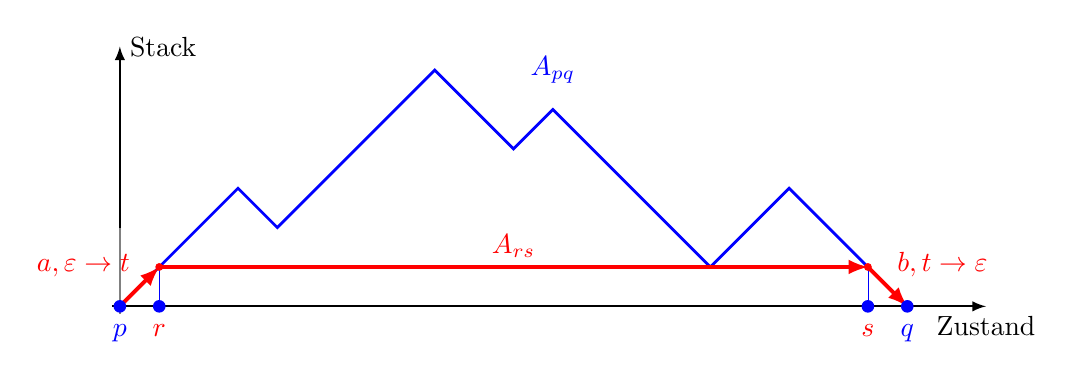
\begin{tikzpicture}[>=latex]

\draw[->,line width=0.7pt] (-0.1,0)--(11.0,0) coordinate[label={below:Zustand}];
\draw[line width=0.7pt,color=gray] (0,-0.1)--(0,1.3);
\draw[->,line width=0.7pt] (0,1.0)--(0,3.3) coordinate[label={right:Stack}];

\draw[color=blue,line width=1pt]
	  ( 0.0,0.0)
	--( 1.5,1.5)
	--( 2.0,1.0)
	--( 4.0,3.0)
	--( 5.0,2.0)
	--( 5.5,2.5)
	--( 7.5,0.5)
	--( 8.5,1.5)
	--(10.0,0.0);

\draw[->,color=red,line width=1.4pt] (0,0)--(0.5,0.5);
\draw[->,color=red,line width=1.4pt] (0.5,0.5)--(9.5,0.5);
\draw[->,color=red,line width=1.4pt] (9.5,0.5)--(10.0,0.0);

\draw[line width=0.1pt,color=blue] (0.5,0.5)--(0.5,0.0);
\draw[line width=0.1pt,color=blue] (9.5,0.5)--(9.5,0.0);

\fill[color=red] ( 0.5,0.5) circle[radius=0.05];
\fill[color=red] ( 9.5,0.5) circle[radius=0.05];

\fill[color=blue] ( 0.0,0.0) circle[radius=0.08];
\fill[color=blue] ( 0.5,0.0) circle[radius=0.08];
\fill[color=blue] ( 9.5,0.0) circle[radius=0.08];
\fill[color=blue] (10.0,0.0) circle[radius=0.08];

\node[color=blue] at ( 0.0,0.0) [below] {$\mathstrut p$};
\node[color=red] at ( 0.5,0.0) [below] {$\mathstrut r$};
\node[color=red] at ( 9.5,0.0) [below] {$\mathstrut s$};
\node[color=blue] at (10.0,0.0) [below] {$\mathstrut q$};

\node[color=red] at (5.0,0.5) [above] {$A_{rs}$};
\node[color=red] at (0.25,0.25) [above left] {$a,\varepsilon\to t$};
\node[color=red] at (9.75,0.25) [above right] {$b,t\to\varepsilon$};

\node[color=blue] at (5.5,3) {$A_{pq}$};

\end{tikzpicture}
